\section{Preliminary}
\subsection{Problem Description}
Suppose there are $n$ voters, indexed by numbers $1,2,...,n$, and $m$ candidates, indexed by capital letters $A,B,C,...$. We separate the liquid democracy  problem into three periods:
\begin{itemize}
	\item \textbf{Spare period} During spare period, no voting  is hold. Each voter can arbitrarily delegate, undelegate and change delegate, by sending a massage (transaction) to the blockchain, which is stored in the delegate contract. Each voter is allowed to appoint at most one delegate. 
	\item \textbf{Prepare period}
	In prepare period, a specific voting is to be hold. The holder needs to deploy the voting contract and the delegate graph and each voters voting powers need to be constructed. In the following example we regard the delegate graph as input,  while in the next section we will show how the voting powers are determined and how to handle the case where there is a cycle in the delegate graph. %and return a no-loop graph.
	\item \textbf{Voting period} After the voting begins, each voter can directly vote to a candidate by sending a voting message, with all his delegators' voting powers also cast to that candidate (which may also reduce the vote of the candidate that his delegate votes). The on-chain voting status are updated for each voting message and need to be displayed. For convenience, we assume that each voter can only vote once during each voting activity, while our algorithm also fits for the case where each voter can change his vote. A voter's delegate is not allowed to change during voting period.
\end{itemize}
It is notable that, although our algorithm does not allow voters to change their delegates during the voting period, they can accomplish the same thing by casting a direct vote.  Changing delegate to a voter that has voted is equivalent to casting a direct vote and changing delegate to a voter that has not voted is rare in practice. Actually, a voter wants to change his delegate during the voting period usually because  he dislikes the way his delegate votes, which means that he has a better candidate in mind and is better off to vote by himself, and he has the time to do so.

The following example abstracts how voting status changes upon receiving voting massages during voting  period.
%Suppose there are $n$ voters, each voter has a certain amount of voting power $a[i],i=1,2,...,n$.
%The liquid democracy refers that, each voter (called delegator) can delegate all his voting power to another voter (called delegatee), and his degegatee can further delegate all those voting power to another delegatee. Whenever a delegatee votes to a candidate, by default, all his delegators' (including multi-level) voting powers are also cast to that candidate.
 Suppose a (direct, no-cycle) delegate graph $G=(V,E)$ is given, where each node represents a voter, and a direct edge $(u,v)$ represents that voter $v$ delegates to voter $u$. We will use terms ``voter" and ``node" interchangeably in the following of this paper.  Since by assumption there is no
cycle in $G$, thus $G$ is a forest (multiple trees). For convenience, we add a virtual node (indexed 0) that
is pointed by the root of each connected branch. So $G$ is transferred to tree $T$, as
Figure~\ref{fig:1}. That is, there are 12 voters. We further assume that each voter's voting power equals to his index. 

\begin{itemize}
\item At the beginning, nobody
votes. When voter 1 votes for candidate $A$ (as the first voter), $A$ obtains
$1+2+...+12=78$ votes.

\item After voter 1 votes, suppose voter 5 (as the second
voter) votes for candidate $B$. Then $B$ obtains $6+5=11$ votes. $A$'s vote
decreases by 11, turning into 67.

\item Further, voter 3 (as the third voter) votes for candidate $C$, then $C$
obtains $3+4+7+8=22$ votes, $A$'s vote becomes 45, and $B$'s vote is still 11.
\end{itemize}

\begin{figure*}
  \centering
  \begin{tikzpicture}
%\tikzset{grow'=right,level distance=32pt}
%\tikzset{execute at begin node=\strut}
%\tikzset{every tree node/.style={anchor=base west}}
\Tree
[.\node[fsn](n1){1};
  [.\node[sn]{2};
   [.\node[sn]{3};
    [.\node[sn]{4};
     [.\node[fsn](n5){5};
      [.\node[sn]{6};]]]
    [.\node[sn]{7};
     [.\node[sn](n8){8};]]] ]
  [.\node[sn]{9};
   [.\node[sn]{10};]
   [.\node[sn]{11};]
   [.\node[sn]{12};]]
]
\node (a) at ($(n1.east) + (1, 0)$) {A};
\node (b) at ($(n5.west) + (-1, 0)$) {B};
\draw [->, >=stealth', color=blue] (n1) -- (a);
\draw [->, >=stealth', color=blue] (n5) -- (b);

\end{tikzpicture}

  	\caption{Tree $T$. We ignore the virtual node with index 0 here.}
  		\label{fig:1}
\end{figure*}
\textbf{Goal}:
For each voting massage, display the votes of all candidates. (Suppose $m<100$)

\begin{tabular}{|c|c|}
input & output \\
1 A			&		A 78 B 0 C 0
\\
5 B			&		A 67 B 11 C 0
\\
3 C			&		A 45 B 11 C 22
\end{tabular}
\subsection{Blockchain and Smart Contract}
The smart contract of Ethereum supports Turing-complete programming language, which is deployed on the blockchain \cite{bocek2018smart}. Users invoke a smart contract by sending a transaction to the smart contract's address, which contains additional information including the gas fee of the transaction and other incoming parameters, which would further be included in a block. As shown in section 1, the gas fee of a valid transaction are limited by the fixed parameter block\_gas\_limit, so that the number of instructions of the smart contract are also bounded. That is the so-called "on-chain" time complexity. In this paper, we use ``voting massage" to represent the transaction that invokes the voting contract, whose on-chain time complexity are required to be sub-linear to the number of voters.  Ethereum clients obtain latest on-chain data through P2P network and implement smart contracts locally through the Etheruem virtual machine (EVM). Thus, the space limitation of a smart contract only depends on Ethereum nodes' (clients) local storage, which is not an issue in this paper.

It is important to distinguish on-chain smart contract and (open source) cloud computation. The later is still realized by centralized servers, which can not guarantee the codes are correctly executed, while in Ethereum, there is no "center" for executing smart contract: they are executed by every Ethereum node, which is reliable as long as the majority of nodes are honest.

\subsection{Merkel Tree}
The Merkel Tree is a common used method for store and verifying on-chain data. One of the key tools is the hash function, $h()$, which is (cryptographically) hard to find collisions and for inverse computation (In Ethereum, SHA3-256 is used). The Merkel tree is a full binary tree, where each leaf node stores the hash value of data to be stored (see Figure \ref{fig:merkel}). The value of an intermediate node is the hash value of the combination of its two children. 
\begin{figure*}
	\centering
	\label{fig:merkel}
	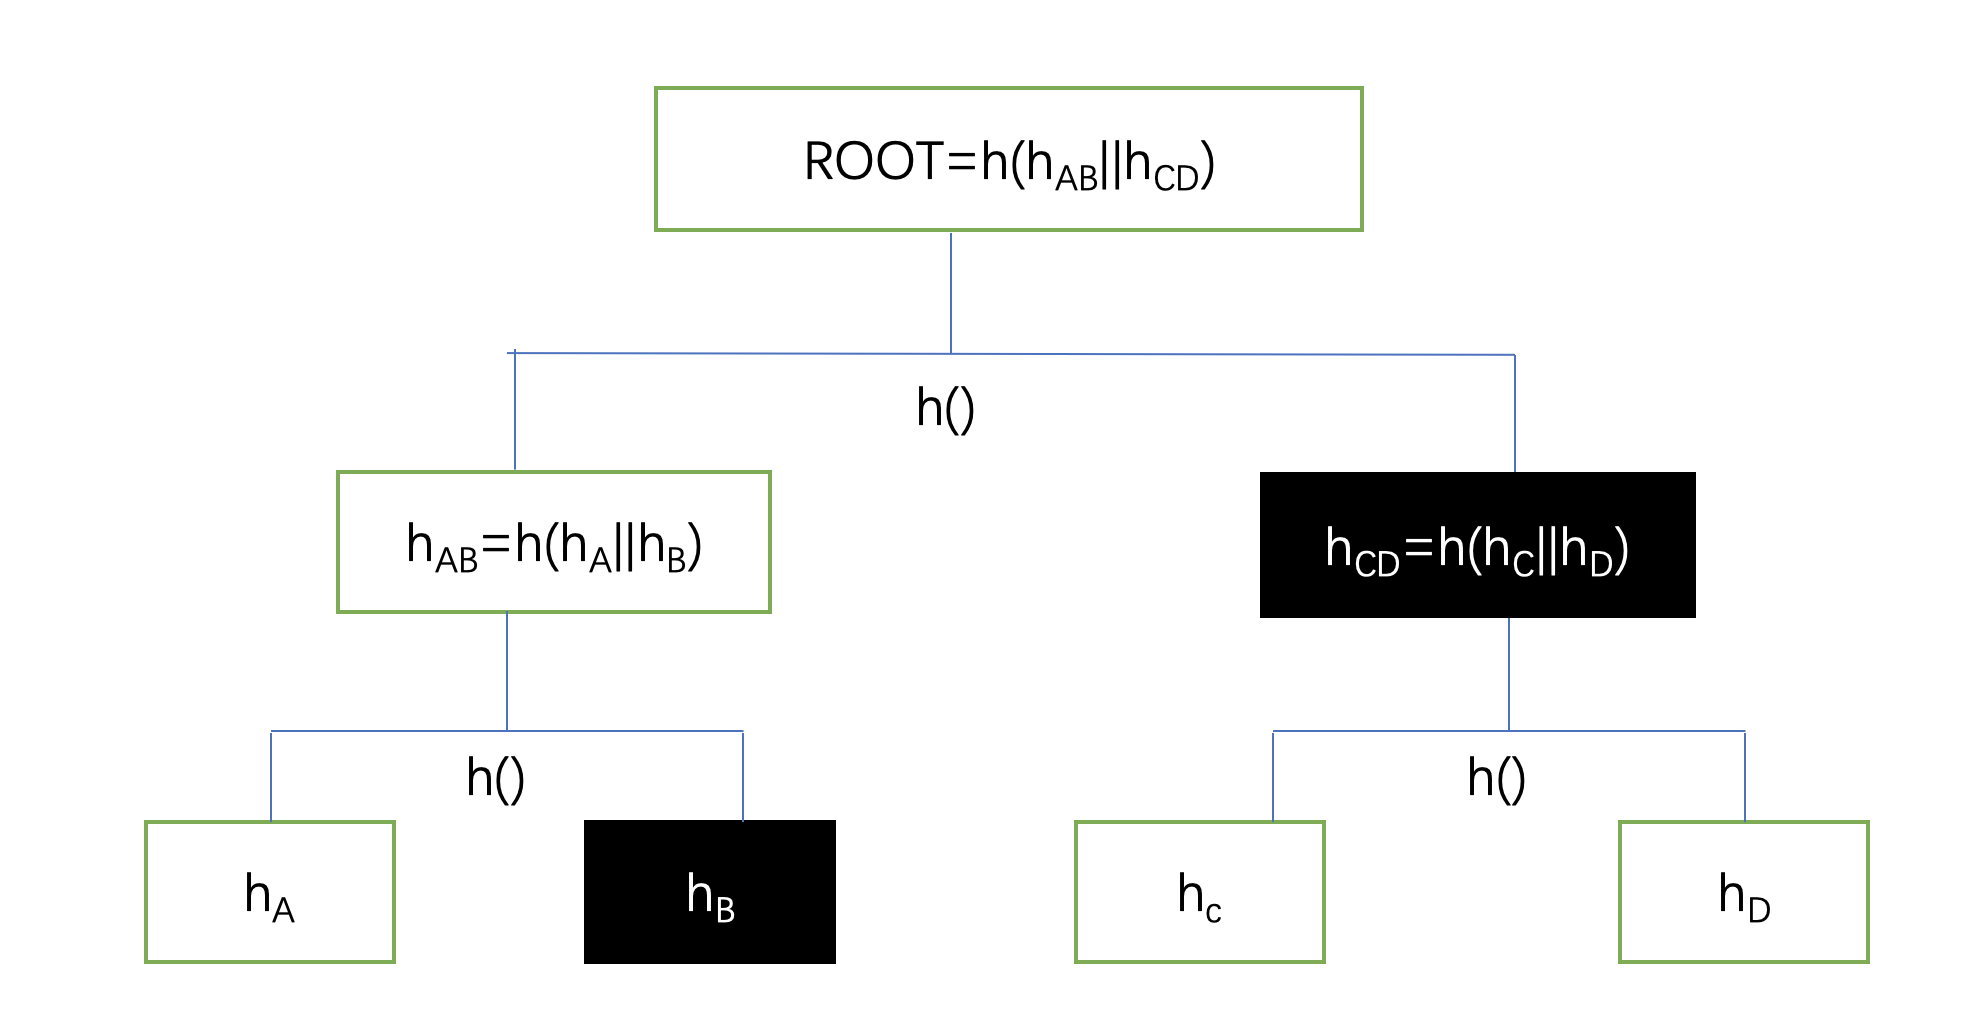
\includegraphics[width=1.1\textwidth]{merkel.png}
	%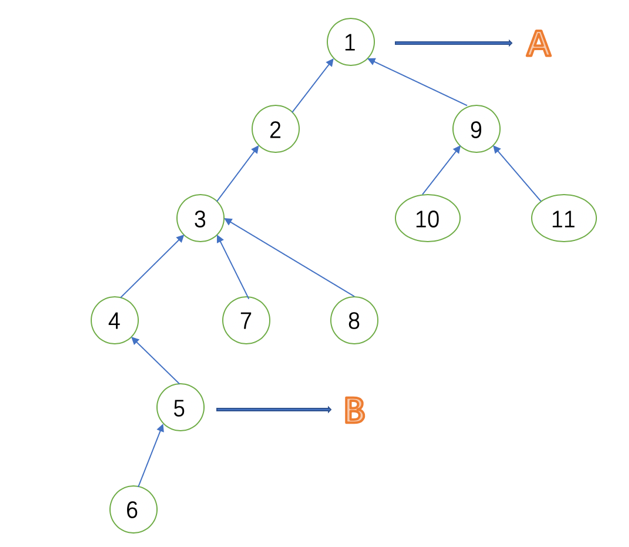
\includegraphics[width=0.6\textwidth]{2.png}
	\caption{Merkel tree, where $h_{A/B/C/D}$ refers to the hash value of data $A/B/C/D$. The black nodes represent the Merkel path of data $A$.}
\end{figure*}

The use of Merkel tree is that, the blockchain only need to store the root of the Merkel tree. In order to proof that a data (say data $A$ in the Figure \ref{fig:merkel})belongs to the Merkel tree, $A$ along with its Merkel path (also called Merkel Proof) are required:

\textbf{Merkel path}, which is defined to be a sequence of nodes in the Merkel tree that corresponds to brother of each node on path from  $A$'s leaf node to the root. For example, data $A$'s Merkel path is $(h_B,h_{CD})$. A leaf node together with its correct Merkel path can recover the root of the Merkel tree (called Merkel root). The length of the Merkel path and the time complexity for recovering the Merkel root are all logarithmic to the number of leaf nodes of the Merkel tree. The one-wayness of the hash function guarantees that it is hard to construct a correct Merkel path for any data that does not belong to any leaf nodes of the Merkel tree.
\subsection{Interval Tree}
Interval tree is also a binary tree, where each node represents a interval and the interval of a parent node is uniformly distributed to its two child nodes, until the interval becomes a singular, to be a leaf node. 
\begin{figure}
	\centering
	\begin{tikzpicture}[level distance=60pt]
\tikzset{edge from parent/.style=
{draw,
edge from parent path={(\tikzparentnode.south)
-- +(0,-8pt)
-| (\tikzchildnode)}}}
%\tikzset{grow'=right,level distance=32pt}
%\tikzset{execute at begin node=\strut}
%\tikzset{every tree node/.style={anchor=base west}}
\Tree
[.\node[kn](n1){{\color{blue}1}\\$[1,12]$};
  [.\node[kn]{{\color{blue}2}\\$[1,6]$};
   [.\node[kn]{{\color{blue}4}\\$[1,3]$};
    [.\node[kn]{{\color{blue}8}\\$[1,2]$};
     [.\node[kn]{{\color{blue}16}\\$[1,1]$};]
     [.\node[kn]{{\color{blue}17}\\$[2,2]$};]
    ]
    [.\node[kn]{{\color{blue}9}\\$[3,3]$};]
   ]
   [.\node[kn]{{\color{blue}5}\\$[4,6]$};
    [.\node[kn]{{\color{blue}10}\\$[4,5]$};
     [.\node[kn]{{\color{blue}20}\\$[4,4]$};]
     [.\node[kn]{{\color{blue}21}\\$[5,5]$};]
    ]
    [.\node[kn]{{\color{blue}11}\\$[6,6]$};]
   ]
  ]
  [.\node[kn]{{\color{blue}3}\\$[7,12]$};
   [.\node[kn](n6){{\color{blue}6}\\$[7,9]$};]
   [.\node[kn](n7){{\color{blue}7}\\$[10,12]$};]]
]

\node (a) at ($(n6.south) + (0, -0.5)$) {...};
\node (b) at ($(n7.south) + (0, -0.5)$) {...};
\end{tikzpicture}

	\caption{The interval tree of all nodes}
				\label{fig:interval}
\end{figure}
See Figure \ref{fig:interval} for the interval tree of the 12 nodes in Figure \ref{fig:1}. The root are indexed 1 and for node $k$, its child nodes are indexed $2k,2k+1$ respectively. Note that, although some indexes, e.g. 18,19 in Figure \ref{fig:merkel}, does not exist, the space is still used. 

Interval tree is usually used for maintaining an array where the operations are aiming at a successive interval. Given the interval to be updated, the execution begins at the root node, then the interval are separated to one or two sub-intervals. which are recursively executed at the child notes, guaranteeing that the sub-intervals to be update belongs to interval of current node. The recursion ends when the interval to be update equals to the interval of current node. For example, when interval 
[4,8] is to be update, beginning at the root, it separates to [4,6] and [7,8], which are executed at note 2 and 3 respectively. The recursion ends at node 5 and node 12 (which are omitted in Figure \ref{fig:interval}).

Interval tree supports find and update operation. For update operation, usually not every leaf node is updated since the update information may stop at an intermediate node, recorded as lazy-tag, which means that it is temporarily suspended and will be executed in subsequent operations. Find operations need to be executed recursively starting from the root, and trigger the pass-down operation of all lazy-tags until the leaf node is reached. The complexity is $O(\log n)$ with respect to interval tree for both operations. We refer \cite{mulmuley1994computational}, Chapter 10.1 to readers for more detail.


